\section{Derivation}
To derive the modelling equations for the Cubli system from Newton's Second Law, the former is split up into its two moving parts as seen in \figref{freeBodyFrame} and \figref{freeBodyWheel}.

  \begin{minipage}{\linewidth}
  	\begin{minipage}{0.45\linewidth}
  		\begin{figure}[H]
  			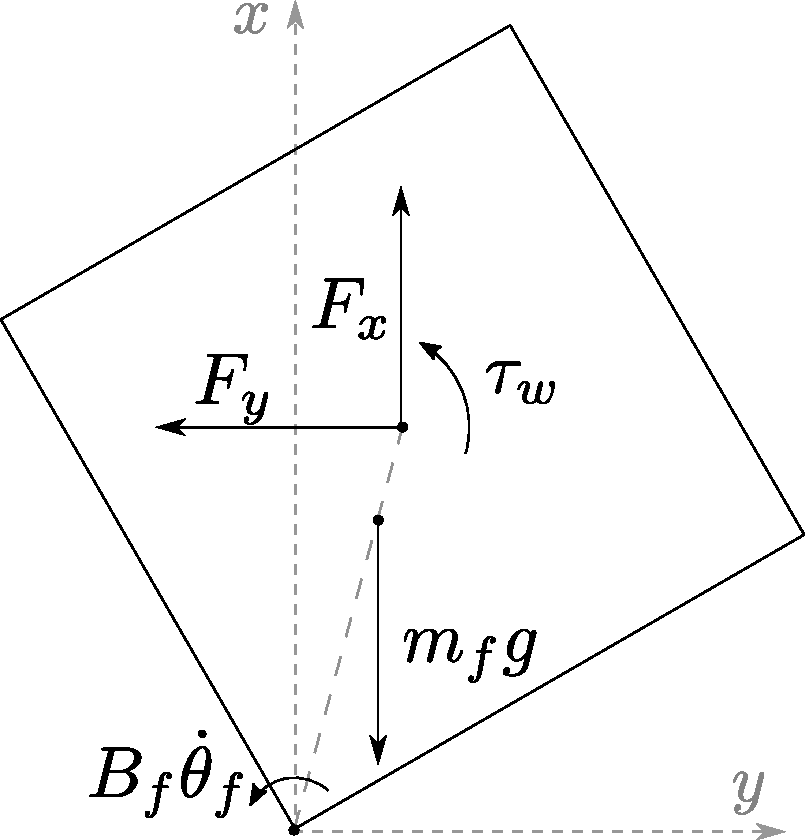
\includegraphics[scale=.5]{figures/freeBodyFrame}
  			\centering
  			\captionsetup{justification=centering}
  			\captionof{figure}{\\Free body diagram of the frame of the Cubli}
  			\label{freeBodyFrame}
  		\end{figure}\vspace{-5mm}
  	\end{minipage}
  	\hspace{0.03\linewidth}
  	\begin{minipage}{0.45\linewidth}
  		\begin{figure}[H]
  			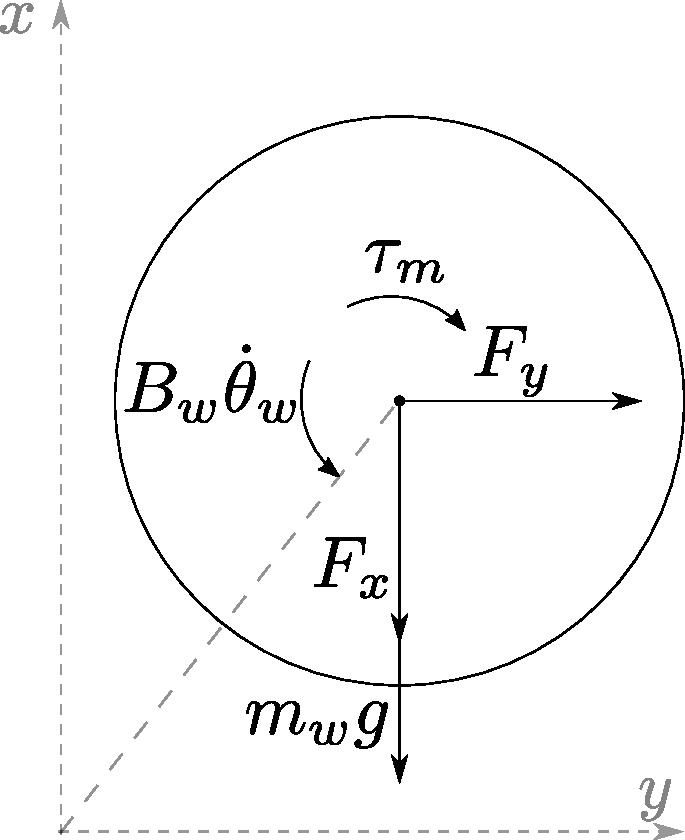
\includegraphics[scale=.53]{figures/freeBodyWheel}
  			\centering
  			\captionsetup{justification=centering}
  			\captionof{figure}{\\Free body diagram of the reaction wheel of the Cubli}
  			\label{freeBodyWheel}
  		\end{figure}\vspace{-5mm}
  	\end{minipage}
  \end{minipage}

The equation for the frame is deduced from the \figref{freeBodyFrame}.
\begin{flalign}
  \eq{J_F \vec{\ddot{\theta}_F}} { -B_F \vec{\dot{\theta}_F} + \vec{l_F} \times (m_F\cdot \vec{g}) + \vec{l_w} \times \vec{F} - \vec{\tau_m} + B_w \vec{\dot{\theta}_w}} \unit{N\cdot m}
\label{frameModelEq}
\end{flalign}
%
\hspace{6mm} Where:\\
\begin{tabular}{ p{1cm} l l l}
& \si{J_F} 					    	   & is the inertia of the frame                          &\unitWh{kg \cdot m^2} \\
& \si{\vec{\ddot{\theta}_F}} & is the angular acceleration of the frame             &\unitWh{rad \cdot s^{-2}} \\
& \si{B_F} 	                 & is the friction coefficient of the frame             &\unitWh{N \cdot m \cdot s \cdot rad^{-1}} \\
& \si{\vec{\dot{\theta}_F}}  & is the angular velocity of the frame                 &\unitWh{rad \cdot s^{-1}} \\
& \si{\vec{l_F}}             & is the length to center of mass of the frame         &\unitWh{m} \\
& \si{m_F}                   & is the mass of the frame                             &\unitWh{kg} \\
& \si{\vec{g}}							 & is the gravitational acceleration                    &\unitWh{m\cdot s^{-2}} \\
& \si{\vec{l_w}}             & is the length to center off mass of the wheel        &\unitWh{m} \\
& \si{\vec{F}}				  	   & is the force delivered to the frame from the wheel   &\unitWh{N} \\
& \si{\vec{\tau_m}} 	       & is the torque delivered by the motor        &\unitWh{N \cdot m} \\
& \si{B_w} 	                 & is the friction coefficient of the wheel             &\unitWh{N \cdot m \cdot s \cdot rad^{-1}} \\
& \si{\vec{\dot{\theta}_w}}  & is the angular velocity of the wheel with respect to the frame                 &\unitWh{rad \cdot s^{-1}} \\
\end{tabular}

The following equation is then derived from \figref{freeBodyWheel}:
\begin{flalign}
  \eq{ J_w (\ \vec{\ddot{\theta}_F} + \vec{\ddot{\theta}_w}\ ) } { \vec{\tau_m} - B_w \vec{\dot{\theta}_w }} \unit{N\cdot m }
\label{tauW}
\end{flalign}
\hspace{6mm} Where:\\
\begin{tabular}{ p{1cm} l l l}
& \si{J_w} 					    	   & is the inertia of the wheel                          &\unitWh{kg \cdot m^2} \\
& \si{\vec{\ddot{\theta}_w}} & is the angular acceleration of the wheel with respect to the frame             &\unitWh{rad \cdot s^{-2}} \\
\end{tabular}

In \eqref{frameModelEq} the term \si{\vec{l_w} \times \vec{F}} describes the torque delivered from the wheel to the frame, as it acts around the pivot corner of the frame. The vector \si{\vec{F}} is decomposed into to forces paralell to the axes, \si{F_x} and \si{F_y}, as seen on \figref{freeBodyFrame} and \figref{freeBodyWheel}. To be able to apply Newton's Second Law, expressions for both the x- and y-coordinate describing the position of the center of mass of the wheel are found.
%
\begin{flalign}
  \eq{x} { l_w \cdot cos( \theta_F ) } \unit{ m }\\
  \eq{y} { l_w \cdot sin( \theta_F ) } \unit{ m }
\label{xyCoordinate}
\end{flalign}
%
According to Newton's 2nd law of motion, \si{\sum F = m \cdot a}. Then to find \si{F_x} and \si{F_y}, the acceleration of the point at center of mass of the wheel must be known for both the x- and the y-direction. To achieve this the derivatives of the expressions for x and y in \eqref{xyCoordinate} are derived.
%
\begin{flalign}
  \eq{\dot{x}} { -l_w \cdot sin( \theta_F )\ \dot{\theta}_F } \unit{ m\cdot s^{-1} }\\
  \eq{\ddot{x}} { -l_w \cdot cos( \theta_F )\ {\dot{\theta}_F}^{\ \ 2} - l_w \cdot sin( \theta_F ) \ddot{\theta}_F } \unit{ m\cdot s^{-2} }
\label{xCoordinateDerivatives}
\end{flalign}
%
\begin{flalign}
  \eq{\dot{y}} { l_w \cdot cos( \theta_F )\ \dot{\theta}_F } \unit{ m\cdot s^{-1} }\\
  \eq{\ddot{y}} { -l_w \cdot sin( \theta_F )\ {\dot{\theta}_F}^{\ \ 2} + l_w \cdot cos( \theta_F )\ \ddot{\theta}_F } \unit{ m\cdot s^{-2} }
\label{yCoordinateDerivatives}
\end{flalign}
%
\Eqref{xCoordinateDerivatives} and \eqref{yCoordinateDerivatives} can now be used with Newton's 2nd law of motion, while also taking gravity into account in sum of forces, to derive \si{F_x} and \si{F_y}.
%
\begin{flalign}
  \eq{ -F_x -m_w \cdot g }{ m_w \cdot \ddot{x} } &\nonumber\\
  \eq{ F_x }{ - m_w \cdot \ddot{x} - m_w \cdot g} &\nonumber\\
  \eq{ F_x }{ m_w \cdot (\  l_w \cdot cos( \theta_F )\ {\dot{\theta}_F}^{\ \ 2} + l_w \cdot sin( \theta_F )\ \ddot{\theta}_F \ ) - m_w \cdot g} \unit{N}
\label{Fx}
\end{flalign}
%
\begin{flalign}
  \eq{ -F_y }{ m_w \cdot \ddot{y} } & \nonumber\\
  \eq{ F_y }{ -m_w \cdot (\ -l_w \cdot sin( \theta_F )\ {\dot{\theta}_F}^{\ \ 2} + l_w \cdot cos( \theta_F )\ \ddot{\theta}_F\ ) } & \nonumber\\
  \eq{ F_y }{ m_w \cdot (\ l_w \cdot sin( \theta_F )\ {\dot{\theta}_F}^{\ \ 2} - l_w \cdot cos( \theta_F )\ \ddot{\theta}_F\ ) } \unit{N}
\label{Fy}
\end{flalign}

The original objective was to evaluate the term \si{\vec{l_w} \times \vec{F}} in \eqref{frameModelEq}. Since the expressions for the two forces, \si{F_x} and \si{F_y}, that compose the vector \si{\vec{F}}, are found in \eqrefTwo{Fx}{Fy}, the vector product from \eqref{frameModelEq} is evaluated.

\begin{flalign}
  \si{\vec{l_w} \times \vec{F}} &=
    \begin{vmatrix}
      \ \si{\vec{\hat{i}}}                & \si{\vec{\hat{j}}}               & \si{\vec{\hat{k}}} \ \ \ \\ 
      \ \si{ l_w \cdot cos( \theta_F ) }  & \si{ l_w \cdot sin( \theta_F ) } & 0                  \ \ \ \\ 
      \ \si{ F_x }                        & \si{ F_y }                      & 0                  \ \ \  
    \end{vmatrix} \unit{N\cdot m}\\ \nonumber \\
  \si{ \vec{l_w} \times \vec{F} } &= 
    \begin{bmatrix}
      \ \si{ ( l_w \cdot sin( \theta_F) \cdot 0 - 0 \cdot F_y ) } \ \ \ \\
      \ \si{ ( l_w \cdot cos( \theta_F )\cdot 0 + 0 \cdot F_x  ) } \ \ \ \\
      \ \si{ ( l_w \cdot cos( \theta_F )\cdot F_y - l_w \cdot sin( \theta_F )\cdot F_x ) }
    \end{bmatrix} \unit{N\cdot m} \\ \nonumber\\
  \si{ \vec{l_w} \times \vec{F} } &= \si{ 0 \cdot \hat{i} + 0 \cdot \hat{j} + ( l_w \cdot cos( \theta_F )\cdot (m_w \cdot (\ l_w \cdot sin( \theta_F )\ {\dot{\theta}_F}^{\ \ 2} - l_w \cdot cos( \theta_F )\ \ddot{\theta}_F\ ))} \nonumber \\
  &\ \ \ \ \si{- l_w \cdot sin( \theta_F )\cdot (m_w \cdot (\  l_w \ cos( \theta_F )\ {\dot{\theta}_F}^{\ \ 2} + l_w \cdot sin( \theta_F )\ \ddot{\theta}_F \ )} \nonumber \\
  &\ \ \ \ \si{- m_w \cdot g) ) \cdot \hat{k}} \unit{N \cdot m}\\ \nonumber\\
  \eq{ \vec{l_w} \times \vec{F} }{ ({-l_w}^2 \cdot m_w \ddot{\theta}_F \ (cos^2(\theta_F) + sin^2(\theta_F)) + l_w\cdot sin(\theta_F)\ m_w \cdot g ) \cdot \hat{k}} \unit{N \cdot m}\\ \nonumber\\
  \eq{ \vec{l_w} \times \vec{F} }{ (-{l_w}^2 \cdot m_w \ddot{\theta}_F + l_w\ sin(\theta_F)\ m_w \cdot g ) \cdot \hat{k}} \unit{N \cdot m}
\label{vectorDecomposition3}
\end{flalign}

Since all torques only have a z-coordinate, \eqref{vectorDecomposition3} is inserted in \eqref{frameModelEq}, without vector-notation. Note that \si{\vec{l_F} \times (m_F\cdot \vec{g}) = (m_F \cdot l_F \cdot g \cdot sin(\theta_F)) \cdot \hat{k} }.
%
\begin{flalign}
	\si{J_F \cdot \ddot{\theta}_F} &= \si{- B_F \cdot \dot{\theta}_F + m_F \cdot l_F \cdot g \cdot sin(\theta_F)} \nonumber\\ 
	&\ \ \ \ \si{- m_w \cdot {l_w}^{2} \cdot \ddot{\theta}_F + m_w \cdot l_w  \cdot g \cdot sin(\theta_F) - \tau_m + B_w \cdot \dot{\theta}_w} \unit{N\cdot m}
\label{FrameEq2}
\end{flalign}
%
\begin{flalign}
	\eq{(J_F+m_w \cdot {l_w}^{2}) \cdot \ddot{\theta}_F} {- B_F \cdot \dot{\theta}_F + (m_F \cdot l_F + m_w \cdot l_w) \cdot g \cdot sin(\theta_F) - \tau_m + B_w \cdot \dot{\theta}_w} \unit{N\cdot m}
\label{FrameEq3}
\end{flalign}

Isolating \si{\ddot{\theta}_F} from \eqref{FrameEq3} gives the final expression for the rotational acceleration of the frame.
\begin{flalign}
	\eq{\ddot{\theta}_F} {\frac{- B_F \cdot \dot{\theta}_F + (m_F \cdot l_F + m_w \cdot l_w) \cdot g \cdot sin(\theta_F) - \tau_m + B_w \cdot \dot{\theta}_w}{J_F + m_w \cdot {l_w}^{2}}}  \unit{rad \cdot s^{-1}} 
\label{FrameEq4}
\end{flalign}

The equation above can be rearranged to clarify the effect that each variable exerts on the final acceleration of the frame.
\begin{flalign}
	\eqOne{\ddot{\theta}_F} {-\frac{B_F}{J_F + m_w \cdot l^2_w} \cdot \dot{\theta}_F + \frac{(m_F \cdot l_F + m_w \cdot l_w) \cdot g}{J_F + m_w \cdot l^2_w} \cdot sin(\theta_F)}
	\eqTwo{ - \frac{1}{J_F + m_w \cdot l^2_w} \cdot \tau_m + \frac{B_w}{J_F + m_w \cdot l^2_w} \cdot \dot{\theta}_w}   \unit{rad \cdot s^{-1}} 
\label{FrameEqFinal}
\end{flalign}

Once the acceleration of the frame is described by \eqref{FrameEqFinal} it is possible to derive an expression for the angular acceleration of the wheel with respect to its axis from \eqref{tauW}.
\begin{flalign}
	\eq{\ddot{\theta}_w} {\frac{\tau_m - B_w \cdot \dot{\theta}_w}{J_w} - \ddot{\theta}_F} \unit{rad \cdot s^{-1}} 
\label{WheelRotEq2}
\end{flalign}

Substituting \si{\ddot{\theta}_F} by the expression for the angular acceleration of the frame (\eqref{FrameEq4}) into \eqref{WheelRotEq2} gives the final description for \si{\ddot{\theta}_w}, as shown in \eqref{WheelRotEqFinal}.
\begin{flalign}
	\si{\ddot{\theta}_w} &= \si{\frac{\tau_m - B_w \cdot \dot{\theta}_w}{J_w}}\nonumber\\ 
	&\ \ \ \ \si{- \frac{(m_F \cdot l_F + m_w \cdot l_w) \cdot g \cdot sin(\theta_F) - \tau_m + B_w \cdot \dot{\theta}_w - B_F \cdot \dot{\theta}_F}{J_F+m_w \cdot {l_w}^{2}}} \unit{rad \cdot s^{-1}}
\label{WheelRotEq3}
\end{flalign}
%
\begin{flalign}
	\eqOne{\ddot{\theta}_w} {\frac{(J_w+J_F+{l_w}^{2} \cdot m_w) \cdot (\tau_m - B_w \cdot \dot{\theta}_w)}{J_w \cdot (J_F+m_w \cdot {l_w}^{2})}}
	\eqTwo{- \frac{(m_F \cdot l_F + m_w \cdot l_w) \cdot g \cdot sin(\theta_F) - B_F \cdot \dot{\theta}_F}{J_F+m_w \cdot {l_w}^{2}}} \unit{rad \cdot s^{-1}}
\label{WheelRotEq4}
\end{flalign}

\Eqref{WheelRotEq4} can be rearranged in the same way as \eqref{WheelRotFinal}.
\begin{flalign}
	\eqOne{\ddot{\theta}_w} {\frac{J_w+J_F+{l_w}^{2} \cdot m_w}{J_w \cdot (J_F+m_w \cdot {l_w}^{2})} \cdot \tau_m - \frac{(J_w+J_F+{l_w}^{2} \cdot m_w) \cdot B_w}{J_w \cdot (J_F+m_w \cdot l_w^{2})} \cdot \dot{\theta}_w }
	\eqTwo{- \frac{(m_F \cdot l_F + m_w \cdot l_w) \cdot g}{J_F+m_w \cdot {l_w}^{2}} \cdot sin(\theta_F) + \frac{B_F}{J_F+m_w \cdot {l_w}^{2}} \cdot \dot{\theta}_F} \unit{rad \cdot s^{-1}} 
\label{WheelRotFinal}
\end{flalign}

The final model of the system can be summarize with the following equations:

\footnotesize{\si{\ddot{\theta}_F = -\frac{B_F}{J_F + m_w \cdot {l_w}^2} \cdot \dot{\theta}_F + \frac{(m_F \cdot l_F + m_w \cdot l_w) \cdot g}{J_F + m_w \cdot {l_w}^2} \cdot sin(\theta_F) - \frac{1}{J_F + m_w \cdot {l_w}^2} \cdot \tau_m + \frac{B_w}{J_F + m_w \cdot {l_w}^2} \cdot \dot{\theta}_w} 	} \begin{flalign} \label{finalFrame} \end{flalign}
%
\footnotesize{\si{\ddot{\theta}_w = \frac{J_w+J_F+m_w \cdot {l_w}^{2}}{J_w \cdot (J_F+m_w \cdot {l_w}^{2})} \cdot \tau_m - \frac{(J_w+J_F+{l_w}^{2} \cdot m_w) \cdot B_w}{J_w \cdot (J_F+m_w \cdot  {l_w}^2)} \cdot \dot{\theta}_w - \frac{(m_F \cdot l_F + m_w \cdot l_w) \cdot g}{J_F+m_w \cdot {l_w}^{2}} \cdot sin(\theta_F) + \frac{B_F}{J_F+m_w \cdot {l_w}^{2}} \cdot \dot{\theta}_F}} \begin{flalign} \label{finalWheel} \end{flalign}
%
\fxnote{allign more beautifully}